\documentclass[10pt]{beamer}
\hypersetup{pdfpagemode=FullScreen}
\usetheme{CambridgeUS}
\usecolortheme{default}
\usefonttheme{serif}
\setbeamertemplate{navigation symbols}{}
\usepackage{microtype}
\usepackage{graphicx}
\usepackage{mathtools}
\usepackage{breqn}
\usepackage{empheq}
\usepackage{tensor}
\usepackage{array}
\usepackage{multirow}
\usepackage{transparent}
\usepackage{booktabs}
\usepackage{natbib}
\usepackage{hyperref}
\usepackage[vietnamese]{babel}
\usepackage{setspace}

% Dùng font hệ thống với XeLaTeX hoặc LuaLaTeX
\usepackage{fontspec} % gói này thay thế cho inputenc và fontenc
\setmainfont{Source Sans Pro} % Bạn có thể thay bằng font khác tùy chọn


% set colors
\definecolor{myNewColorA}{RGB}{39,52,139}
\definecolor{myNewColorB}{RGB}{183, 183, 183}
\definecolor{myNewColorC}{RGB}{183, 183, 183}
\setbeamercolor*{palette primary}{bg=myNewColorA, fg=white}
\setbeamercolor*{palette secondary}{bg=myNewColorB, fg=black}
\setbeamercolor*{palette tertiary}{bg=myNewColorB, fg=black}
\setbeamercolor*{titlelike}{fg=myNewColorA}
\setbeamercolor*{title}{bg=myNewColorA, fg=white}
\setbeamercolor*{item}{fg=myNewColorA}
\setbeamercolor*{caption name}{fg=myNewColorA}


% define envoirenmemt
\newenvironment{tres important}[2][]{
	\setkeys{EmphEqEnv}{#2}
	\setkeys{EmphEqOpt}{box={\setlength{\fboxsep}{10pt}\fcolorbox{myNewColorA}{white}},#1}
	\EmphEqMainEnv}
{\endEmphEqMainEnv}
%------------------------------------------------------------

\titlegraphic{
\includegraphics[height=2.5cm]{assets/HUS_MIM_Logo.jpg}}

% To use the other logo of University use following: .......
%\titlegraphic{\includegraphics[height=3cm]{figures/UWA_V_logo.png}}

\setbeamerfont{title}{size=\large}
\setbeamerfont{subtitle}{size=\small}
\setbeamerfont{author}{size=\large}
\setbeamerfont{date}{size=\small}
\setbeamerfont{institute}{size=\large}
\title[CLP with Ant Colony Optimization]{\textbf{ACO cho bài toán Tải Container(CLP)}}
\subtitle{Ant Colony Optimization for Container Loading Problem }
\author[Nhóm 3]{N.Tiến Đạt \quad N.Thành Trung \quad N.Thị Ánh}
\institute[]{}
\date[10/10/2024]

%------------------------------------------------------------
%This block of commands puts the table of contents at the 
%beginning of each section and highlights the current section:
\AtBeginSection[]
{
  \begin{frame}
    \frametitle{Nội dung}
    \tableofcontents[currentsection]
  \end{frame}
}

%------------------------------------------------------------

\begin{document}

%The next statement creates the title page.
%\frame{\titlepage}
        \begin{frame}
            \titlepage
        \end{frame}

        % \begin{frame}
        %     \frametitle{Nội dung}
        %     \tableofcontents    
        % \end{frame}

%------------------------------------------------------------

    \section{Giới thiệu về bài toán CLP}

        \begin{frame}{Bài toán CLP}
            Bài toán Container Loading Problem (CLP) liên quan đến việc sắp xếp một tập hợp các hộp hình chữ nhật ba chiều có kích thước khác nhau vào một container ba chiều có kích thước cố định, sao cho tận dụng không gian trong container một cách tối ưu nhất. 

            \begin{center}
                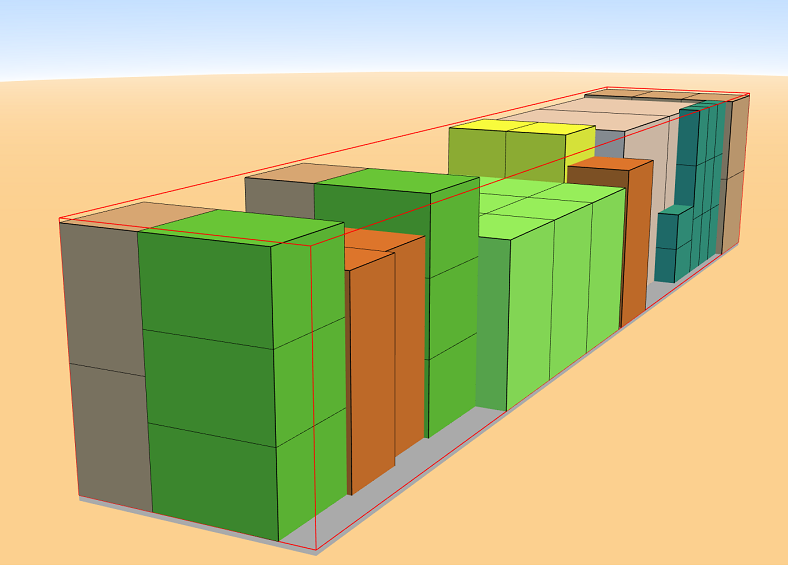
\includegraphics[width=0.55\textwidth]{assets/IntroForCLP_FirstPic.png}
            \end{center}
            \[{\textbf{Fig 1}: \text{Bins and Items in Container}}\]
        \end{frame}

        \begin{frame}{Bài toán CLP}
            CLP có thể được phân loại dựa trên một số tiêu chí (theo Dyckhoff, 1990; Wascher et al., 2007). Đầu tiên, bài toán có thể phân biệt giữa hai dạng:
            \pause %
            \begin{itemize}
                \item \textbf{Dạng ba lô ba chiều (3D knapsack problem):} Cho phép bỏ lại một số hộp nếu cần thiết.
                \item \textbf{Dạng đóng gói (3D bin-packing problem):} Yêu cầu phải xếp toàn bộ các hộp vào container.
            \end{itemize}
            \vspace{0.5cm}
            \pause %
            Bài toán cũng có thể phân loại dựa trên số loại hộp khác nhau, bao gồm:
            \pause %
            \begin{itemize}
                \item \textbf{Bài toán đồng nhất:} Chỉ có một loại hộp duy nhất.
                \item \textbf{Bài toán dị tính yếu (The weakly 
heterogeneous problem):} Có ít loại hộp nhưng số lượng lớn mỗi loại.
                \item \textbf{Bài toán dị tính mạnh ( the strongly 
heterogeneous problem):} Có nhiều loại hộp khác nhau, nhưng số lượng ít mỗi loại.
            \end{itemize}
        \end{frame}

        \begin{frame}{Bài toán CLP}
            \begin{center}
                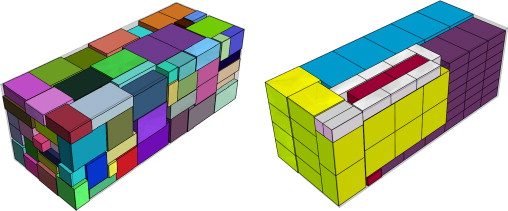
\includegraphics[width=0.9\textwidth]{assets/IntroForCLP_SecondPic.jpg}
            \end{center}
            \[{\textbf{Fig 2}: \text{The weakly and strongly heterogeneous box}}\]
            \[{\textbf{Source}: \text{A biased random key genetic algorithm for 2D and 3D bin packing }}\]
            \[\text{problems, Jos ́e Fernando Gon ̧calves, Mauricio G.C. Resende, 2013, International}\]
            \[\text{ Journal of Production Economics 145(2):500-510}\]
        \end{frame}

        \begin{frame}{Frame Title}
            
        \end{frame}

        \begin{frame}{Bài toán CLP}
            Bài toán \textbf{Container Loading Problem (CLP)} được định nghĩa như sau:
            \vspace{0.08cm}
            
            \begin{spacing}{1.5}
                \textit{
                    "Cho một tập hợp gồm $n$ loại hộp hình chữ nhật ba chiều, mỗi loại $j \in \{1, 2, ..., n\}$ có chiều cao $h_j$, chiều rộng $w_j$, chiều dài $l_j$ và số lượng $m_j$. Container hình chữ nhật có kích thước chiều cao $H$, chiều rộng $W$, và chiều dài $L$. Mục tiêu là sắp xếp một tập hợp con các hộp vào container sao cho tối ưu hóa việc sử dụng không gian container và đáp ứng các ràng buộc bổ sung nếu có."}
            \end{spacing}
        \end{frame}

        \begin{frame}{Bài toán CLP}
            Mục tiêu chính của bài toán CLP là tìm tỷ lệ sử dụng không gian (Space Utilization Ratio - SUR) tốt nhất, được mô tả bởi phương trình sau:

            \[
            \text{max SUR} = \frac{\sum_{a=1}^{b} V_a}{C}, \tag{1}
            \]
            
            Trong đó:
            \begin{itemize}
                \item $b$ = Số lượng hộp đã được sắp xếp
                \item $V_a$ = Thể tích của hộp thứ $a$
                \item $C$ = Thể tích của container
            \end{itemize}
        
        \end{frame}

        \begin{frame}{Frame Title}
            \begin{center}
                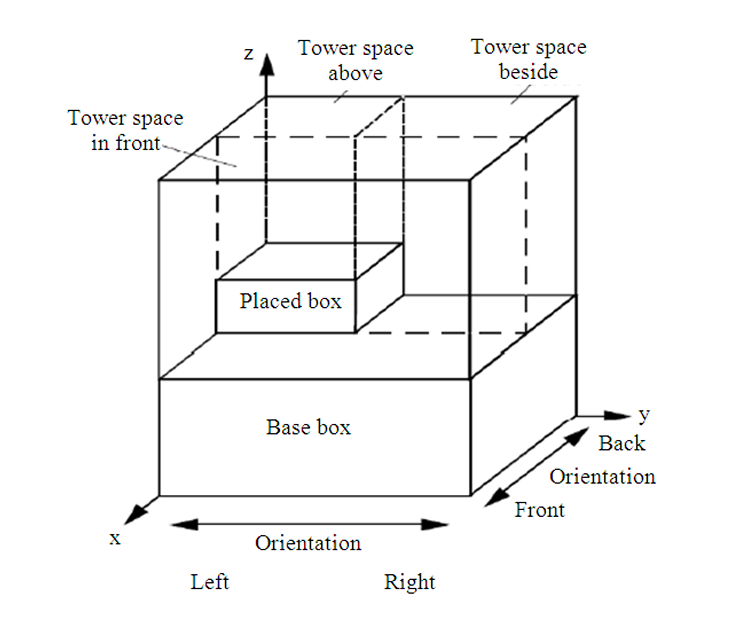
\includegraphics[width=0.6\textwidth]{assets/IntroForCLP_ThirdPic.png}
            \end{center}
        \end{frame}

    \section{Theoretical framework}

    \section{methodology}

    \section{Conclusion}

\end{document}